\documentclass{article}
\usepackage{graphicx} % Required for inserting images

% remove equation auto numbering
\usepackage{amsmath}

% plot functions
\usepackage{pgfplots}
\pgfplotsset{compat = newest}

% make enumeration start from 0
\usepackage{enumitem}

% max 20 ampersand in matrix rows
\setcounter{MaxMatrixCols}{20}

\title{Q $\&$ A}
\author{Daniel Gigliotti}
\date{}

\begin{document}

\maketitle

\newpage

\section{Describe the laplacian of gaussian filter.}

Edges are sudden changes (discontinuities) in the intensity or color of an image, and often highlight important features. Furthermore, they are a more compact representation than pixels. We recall that. We would want to find edges in an efficient manner. How could we find discontinuities? \\

Since images can be seen as a function, we can take its derivative: \textbf{derivatives are large at discontinuities}. Being an image a discrete 2D signal, we will have 2 derivatives, one with respect x and one with respect y. This is called image gradient, a generalization of the concept of derivative to more than one dimension. Image gradients are a representation of the rate of change in the intensity or color of an image in a particular direction. Edges can be traced in the direction perpendicular to the gradient direction, that points in the direction where intensity increase the most. \\

We can get the gradient of an image by applying derivative filters, such as the horizontal and vertical Sobel filters. After that, to highlight an edge, we look for the maximum in the gradient magnitude (derivatives are large at discontinuities). We also recall that, when using derivative filters, it is critical to blur the image first in order to reduce the noise. \\

We have room for improvement: instead of using a first derivative filter and looking for the maximum, we can use a second derivative filter (laplacian) and look for zero crossing; it is easier to search for a zero than to find a maximum. Instead of convolving the image with the kernel (like a Gaussian kernel, to smooth it) and \textbf{then} taking the derivative (expensive operation since the derivative is taken with respect to the whole image), we can first compute the derivative of the filter (small) and then convolve it with the image. This is why we talk about the laplacian of gaussian filter. \\

\textbf{In general, the Laplacian filter is used to detect the edges in the images. It don't behave well on noisy images since it amplifies the noise. For this reason we use a Gaussian filter on the noisy image to smooth it and subsequently use the Laplacian filter for edge detection. These two steps are combined, like said above, in a single step when using a laplacian of gaussian filter}. \\

\newpage

The laplacian $L(x, y)$ of an image with pixel intensity values $I(x, y)$ is given by:
\begin{equation*}
    L(x, y) = \frac{\delta^2 I}{\delta x^2} + \frac{\delta^2 I}{\delta y^2} 
\end{equation*}

A standard 2D laplacian filter looks like this:

\begin{center}
    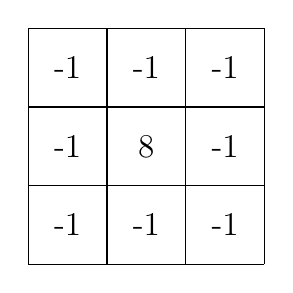
\begin{tikzpicture}
        \draw[step=1cm,color=black] (0, 0) grid (3,3);
        \node[font = {\large}, black] at (0.5, 2.5) {-1};
        \node[font = {\large}, black] at (1.5, 2.5) {-1};
        \node[font = {\large}, black] at (2.5, 2.5) {-1};
        \node[font = {\large}, black] at (0.5, 1.5) {-1};
        \node[font = {\large}, black] at (1.5, 1.5) {8};
        \node[font = {\large}, black] at (2.5, 1.5) {-1};
        \node[font = {\large}, black] at (0.5, 0.5) {-1};
        \node[font = {\large}, black] at (1.5, 0.5) {-1};
        \node[font = {\large}, black] at (2.5, 0.5) {-1};
    \end{tikzpicture}
    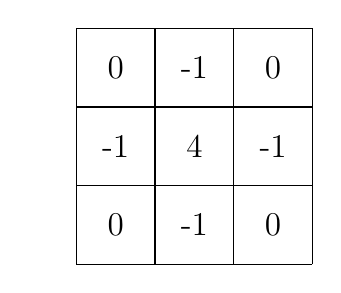
\begin{tikzpicture}
        \draw[step=1cm,color=black] (0, 0) grid (3,3);
        \node[font = {\large}, black] at (0.5, 2.5) {0};
        \node[font = {\large}, black] at (1.5, 2.5) {-1};
        \node[font = {\large}, black] at (2.5, 2.5) {0};
        \node[font = {\large}, black] at (0.5, 1.5) {-1};
        \node[font = {\large}, black] at (1.5, 1.5) {4};
        \node[font = {\large}, black] at (2.5, 1.5) {-1};
        \node[font = {\large}, black] at (0.5, 0.5) {0};
        \node[font = {\large}, black] at (1.5, 0.5) {-1};
        \node[font = {\large}, black] at (2.5, 0.5) {0};

        \node[font = {\large}, black] at (-0.5, 1.5) {};
    \end{tikzpicture}
\end{center}

\begin{center}
    Laplacian operator with and without diagonals
\end{center}

The 2D LoG function centered on zero and with Gaussian standard deviation $\sigma$ has the form:

\begin{equation*}
    LoG(x,y) = -\frac{1}{\pi\sigma^4}[1 - \frac{x^2 + y^2}{2\sigma^2}]e^{-\frac{x^2 + y^2}{2\sigma^2}}
\end{equation*}

A discrete kernel that approximates this function (for a Gaussian $\sigma = 1.4$) is:

\def\pixelmap{{%
{0, 1, 1, 2, 2, 2, 1, 1, 0},
{1, 2, 4, 5, 5, 5, 4, 2, 1},
{1, 4, 5, 3, 0, 3, 5, 4, 1},
{2, 5, 3, -12, -24, -12, 3, 5, 2},
{2, 5, 0, -24, -40, -24, 0, 5, 2},
{2, 5, 3, -12, -24, -12, 3, 5, 2},
{1, 4, 5, 3, 0, 3, 5, 4, 1},
{1, 2, 4, 5, 5, 5, 4, 2, 1},
{0, 1, 1, 2, 2, 2, 1, 1, 0}
}}

\begin{center}
    \begin{tikzpicture}
        [
            box/.style={rectangle,draw=black,thick, minimum size=1cm},
        ]
    
    \foreach \x [count=\i from 0] in {0,1,...,8}
        \foreach \y [count=\j from 0] in {0,1,...,8}
        {
            \def\bit{0}
                \pgfmathsetmacro{\bit}{\pixelmap[\i][\j]}
            %\draw[grid] (\x,-2.5) -- (\x,2.5);
            %\draw[grid] (-2.5,\y) -- (2.5,\y);
            %\fill[cube, color\bit] (\x,\y) -- +(0, 0.25) -- +(.25, .25) -- +(.25,0) -- cycle;
            
            \node[box] at (\x, \y) {\bit};
        }
    
    \end{tikzpicture}
\end{center}

\newpage

\section{Describe Horizontal and Vertical Sobel filters}

One of the earliest and most well-known approaches for edge detection involves the Sobel operators. At the boundary between objects or regions in an image there is usually a rapid shift in pixel intensities. Consequently the magnitude of the derivative at these boundaries tends to be relatively large. Finding the areas in an image with a large derivative can provide insight into the locations of edges and contours. The Sobel operators compute the spatial derivative at each pixel in both x and y direction.

\begin{itemize}
    \item \textbf{Horizontal Sobel filter} $\rightarrow$ when this filter is convolved with an image, it computes the horizontal gradient (it highlights the edges in the image that have a strong change in intensity in the horizontal direction); this means that it can be used to detect edges that are oriented horizontally in the image;
    \begin{center}
        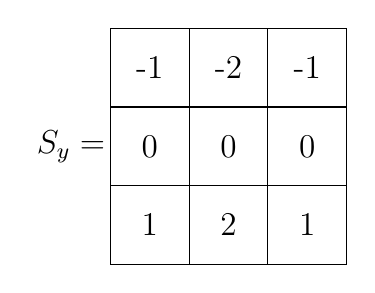
\begin{tikzpicture}
            \draw[step=1cm,color=black] (0, 0) grid (3,3);
            \node[font = {\large}, black] at (0.5, 2.5) {-1};
            \node[font = {\large}, black] at (1.5, 2.5) {-2};
            \node[font = {\large}, black] at (2.5, 2.5) {-1};
            \node[font = {\large}, black] at (0.5, 1.5) {0};
            \node[font = {\large}, black] at (1.5, 1.5) {0};
            \node[font = {\large}, black] at (2.5, 1.5) {0};
            \node[font = {\large}, black] at (0.5, 0.5) {1};
            \node[font = {\large}, black] at (1.5, 0.5) {2};
            \node[font = {\large}, black] at (2.5, 0.5) {1};

            \node[font = {\large}, black] at (-0.5, 1.5) {$S_y = $};
        \end{tikzpicture}
    \end{center}
    \item \textbf{Vertical Sobel filter} $\rightarrow$ when this filter is convolved with an image, it computes the vertical gradient (it highlights the edges in the image that have a strong change in intensity in the vertical direction); this means that it can be used to detect edges that are oriented vertically in the image;
    \begin{center}
        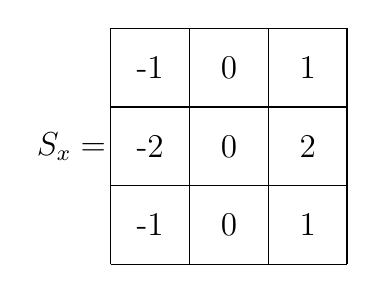
\begin{tikzpicture}
            \draw[step=1cm,color=black] (0, 0) grid (3,3);
            \node[font = {\large}, black] at (0.5, 2.5) {-1};
            \node[font = {\large}, black] at (1.5, 2.5) {0};
            \node[font = {\large}, black] at (2.5, 2.5) {1};
            \node[font = {\large}, black] at (0.5, 1.5) {-2};
            \node[font = {\large}, black] at (1.5, 1.5) {0};
            \node[font = {\large}, black] at (2.5, 1.5) {2};
            \node[font = {\large}, black] at (0.5, 0.5) {-1};
            \node[font = {\large}, black] at (1.5, 0.5) {0};
            \node[font = {\large}, black] at (2.5, 0.5) {1};

            \node[font = {\large}, black] at (-0.5, 1.5) {$S_x = $};
        \end{tikzpicture}
    \end{center}
\end{itemize}

In practice, these two filters are often used together in a technique called \textbf{Sobel edge detection}. By computing the magnitude of the gradient at each pixel using the horizontal and vertical Sobel filters, we can identify the regions in the image where there is a strong change in intensity in any direction, which are likely to correspond to edges in the image. \textbf{This is a rather naive technique}.

\newpage

\section{Why is a Gaussian filter preferred to a box filter? Describe both of them}

The box filter is the simplest kind of filter we can imagine: it simply takes the average of all the pixels under the kernel area. It is linear (it fulfills both the superposition and the homogeneity principles) and separable (can be written as a product of of a column and a row vector). 

By taking the average of the pixels under the kernel area, it smooths out the image, reducing noise. It helps suppressing sharp transitions, however it also tends to blur edges and fine details along with the noise, which may not be desirable in certain applications. \\

The Gaussian filter is another popular choice when it comes to reduce noise and smoothing an image. The Gaussian curve is a bell-shaped function. By convolving it with an image, we give more weight to pixels falling under the center of the filter and less weight to pixels at its edges (weight falls off with distance from center). We can sample the values of a Gaussian function to build a kernel. The size of the kernel may depend on the $\sigma$ value (the standard deviation determines the width of the Gaussian function so choosing the truncation distance based on the standard deviation ensures that the filter considers only the most relevant pixels within a certain distance from the center), or we may want to select the truncating distance as the distance at which the Gaussian function falls to a certain percentage of its maximum value (e.g. $1\%$). The resulting smoothing effect preserves edges and details in the image better than the box filter. \\

Gaussian filter and box filter are two commonly used image smoothing filters in image processing. Although both filters are used for the same purpose of reducing noise and smoothing an image, they produce different results due to their characteristics. \\

The main difference between the two is that the Gaussian filter uses a Gaussian function to compute the weights of the neighboring pixels, giving more weight to the pixels close to the center and decreasing it the more the pixel is far away, while the box filter uses a constant weight for all the pixels in the window. In terms of the output image, this result on a difference in the level of smoothing and blurring that they produce. Applying the box filter results in a uniform smoothing and potential blurring of edges and details in the image. A Gaussian filter instead produces a smoother output image with less blurring compared to a box filter and preserves edges and details. \\

If the goal is to reduce noise and smooth the image while preserving the edges and details, a Gaussian filter is generally preferred. On the other hand, if the goal is to simply reduce noise and blur the image uniformly, a box filter may be more suitable. The choice of the filter depends on the specific application. \\

In the frequency domain, the box filter and the Gaussian filter have different effects on the image:
\begin{itemize}
    \item the \textbf{box filter} has a rectangular frequency response, which lead to a sinc-like function in the spatial domain. The sinc function has oscillations, which can lead to ringing artifacts in the image (ripple-like structures);
    \item the \textbf{Gaussian filter} has a smooth, bell-shaped frequency response. This results in a smoother, more gradual transition between the filtered and unfiltered regions of the image. Gaussian filtering typically produces fewer ringing artifacts than box filtering.
\end{itemize}

Convolving a sinc with an impulse copies the sinc at the location of the impulse. The sinc center lobe causes the blurring, while the outer lobes are responsible for ringing.

\hspace{0.5cm}

\begin{center}
    
    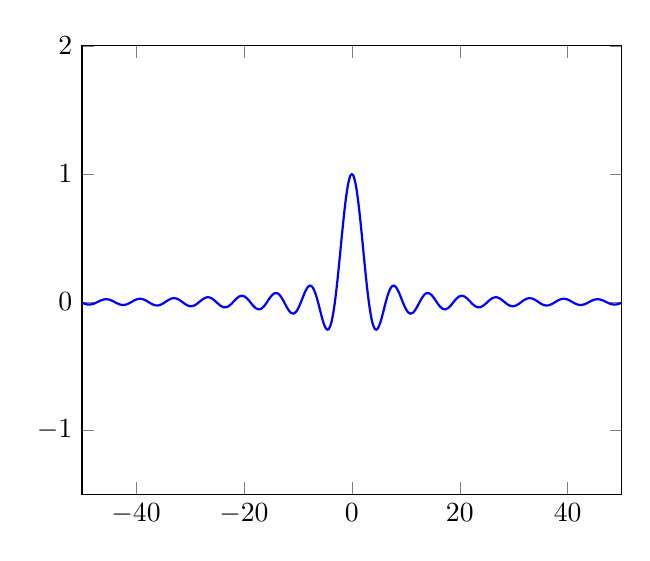
\begin{tikzpicture}
     
    \begin{axis}[
        xmin = -50, xmax = 50,
        ymin = -1.5, ymax = 2.0]
        \addplot[
            domain = -50:50,
            samples = 200,
            smooth,
            thick,
            blue,
        ] {sin(deg(x))) / x};
    \end{axis}
     
\end{tikzpicture}
    
\end{center}

\newpage

\section{Describe the procedure to match image features like SIFT. What are the outliers and how to deal with them?}

Keypoints are distinctive points or locations in an image. Keypoints are typically identified using algorithms like SIFT, SURF, or ORB. The goal of keypoint matching is to establish correspondences between keypoints in different images, enabling further analysis or tasks such as image alignment, object recognition, or 3D reconstruction. \\

The steps typically involve:
\begin{itemize}
    \item \textbf{find all keypoints in a target image}. Each keypoint will have 2D location, scale and orientation. This can be done with various algorithms, such as SIFT, ORB and so on...
    \item \textbf{for each keypoint, search similar keypoints in the other image(s)}.
    \item Once the keypoints are matched, \textbf{they can be used to compute the transformation between the two images}.
\end{itemize}

Feature matching is a broader term that encompasses the matching of not only keypoints but also their associated feature descriptors. Feature descriptors are compact representations of the local image neighborhood around keypoints. Algorithms like SIFT, SURF, and ORB generate both keypoints and feature descriptors. Matching features involves comparing the descriptors of keypoints from one image with those of keypoints from another image to establish reliable correspondences. \\

Given a keypoint/feature in the first image, we can use different techniques to find the best match in the second image:

\begin{itemize}
    \item \textbf{Simple search} with L2 norm:
        \begin{equation*}
            d = | f_1 - f_2 |
        \end{equation*}
        this returns the difference between the features $f_1$ and $f_2$; we need to minimize it in order to find the best match;
    \item \textbf{Distance ratio}:
        \begin{equation*}
            d = \frac{|f_1 - f_2|}{|f_1 - f_2'|}
        \end{equation*}
        \begin{center}
            \textit{$f_2$ is the best match to $f_1$ in $I_2$} \\
            \textit{$f_2'$ is the second best match to $f_1$ in $I_2$}
        \end{center}
        To further improve this method we can \textbf{set the distance ratio threshold ($\rho$) to around $0.5$}, which means that we require our best match to be at least twice as close as our second best match to our initial features descriptor. 
\end{itemize}

After obtaining the initial matches, it's common to encounter outliers, which are incorrect or mismatched feature correspondences due to, for example, noise or changes in lighting conditions. Outliers need to be identified and removed to improve the accuracy of the matching. \\

There are different approaches to deal with outliers. One commonly used technique is RANSAC: RANSAC (RAndom SAmple Consensus) is an iterative algorithm that estimates the parameters of a mathematical model from a set of data containing outliers. In the context of feature matching, RANSAC can be used to estimate a geometric transformation (e.g., homography) between the images by randomly selecting a minimal subset of feature matches and then finding the best transformation that agrees with the majority of inliers. \\

Once the outliers have been identified and removed, the remaining feature matches can be further refined to increase their accuracy. This refinement step may involve methods like bundle adjustment or least squares optimization to improve the alignment between the images.

\newpage

\section{Describe different kind of feature descriptors. In particular, describe the Histogram of Oriented Gradients (HOG) applied to human detection}.

The term \textbf{local feature} refer to distinctive patterns or structures in an image that can be used to identify and describe specific regions of it. Once the local features have been identified and extracted (feature extraction) from an image, they can be used to create a feature vectors that describes the them (feature descriptor). \\

A desirable feature descriptor should possess certain invariance properties to ensure robustness and generalization across different conditions. Here are some common types of invariance that feature descriptors aim to achieve:

\begin{itemize}
    \item \textbf{Scale invariance}: A feature descriptor should be able to detect and describe visual features regardless of their scale. This means that the descriptor should provide consistent representations even when the size of the object or the image changes.
    \item \textbf{Rotation invariance}: An effective feature descriptor should be able to recognize and describe features irrespective of their orientation or rotation in the image. This allows the descriptor to match features that are in different orientations or are subject to rotational transformations.
    \item \textbf{Affine invariance}: Affine transformations include not only rotations but also shearing, scaling, and translation. A desirable feature descriptor should be able to maintain consistency in the feature representation despite these types of transformations.    
    \item \textbf{Illumination invariance}: Lighting conditions can significantly affect the appearance of visual features. A good feature descriptor should be able to provide consistent representations regardless of changes in lighting, ensuring robustness to illumination variations.
\end{itemize}

\newpage

We have various types of feature descriptors. Some naive options include:

\begin{itemize}
    \item \textbf{image gradients}: use the intensity variation between pixels in a window; this way the feature is invariant to absolute intensity changes; \textbf{How can it be less sensitive to deformations?}
    \item \textbf{color histogram}: count the colors in the window using a histogram; this is invariant to changes in scale and rotation; the problem with this approach is that \textbf{we loose spatial information}: two completely different patches with the same colors will have the same descriptor. \textbf{How can we recover spatial information?}
    \item \textbf{orientation normalization}: use the dominant image gradient direction to normalize the orientation of the patch; this is typically achieved by computing the dominant orientation of the image feature and then rotating the image patch; the problem with this approach is that \textbf{the orientation of an image feature can be sensitive to changes in scale}, which can lead to inconsistencies in the descriptor when comparing features at different scales. \textbf{How can we build a descriptor that is invariant (or robust) to scale?}
\end{itemize}

One of the most popular descriptors out there is the Histogram of Oriented Gradients (HOG) descriptor. The Histogram of Oriented Gradients (HOG) descriptor is a widely used feature extraction technique in computer vision. It is particularly effective for object detection and pedestrian recognition tasks. The main steps are:

\begin{itemize}
    \item \textbf{Preprocessing}: preprocess the image to bring down the width to height ratio to 1:2 for ease of computation;
    \item \textbf{Divide the image into $8 \times 8$ patches}. For each patch:
    \begin{itemize}
        \item \textbf{Computing image gradients} for each pixel in the $8 \times 8$ patch;
        \item \textbf{Compute magnitude and orientation} for each pixel in the $8 \times 8$ patch;
        \item \textbf{Generate an weighted orientation histogram} with 9 bins of 20 deg each; this results in a $1 \times 9$ vector describing the patch;
    \end{itemize}
    \item \textbf{Normalize the gradients}: we need to normalize the gradients by taking $16 \times 16$ blocks. Each block has 4 histograms which can be concatenated to form a $1 \times 36$ vector.
    This vector is normalized with L2 norm. It describes the feature that is at the centroid of the $16 \times 16$ block;
    \item Shift the $16 \times 16$ window by 8 pixels and go on. 
\end{itemize}

\newpage

There are two main reasons why the HOG descriptor is so effective in human recognition tasks:

\begin{itemize}
    \item The HOG descriptor \textbf{captures information about the local shape and structure of objects}, which is particularly relevant in human recognition tasks. The arrangement of gradients and their orientations provides a rich representation of edges, corners, and other shape details in the image. Human bodies possess distinctive shapes and contours, and the HOG descriptor is capable of capturing these characteristics effectively.

    \begin{center}
        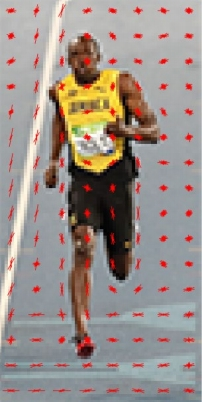
\includegraphics[width=.2\linewidth]{images/human.jpg}    
    \end{center}

    Notice the dominant direction of the histogram captures the shape of the person, especially around the torso and legs.
    
    \item \textbf{Spatial Layout of Features}: The HOG descriptor encodes \textbf{not only the orientation of gradients but also their spatial distribution within predefined cells and blocks}. This spatial layout captures the spatial relationships between different parts of an object. In human recognition tasks, where body parts such as limbs and torsos are crucial for identification, the HOG descriptor's ability to capture spatial information is highly advantageous.

    \item \textbf{Invariance to Geometric Transformations}: The HOG descriptor is relatively invariant to geometric transformations such as translation and scaling. The descriptor's computation involves local image gradients, which are computed relative to the local neighborhood of each cell. This property allows the HOG descriptor to handle variations in pose, scale, and viewpoint, making it suitable for human recognition tasks where people can appear in different orientations and sizes.
\end{itemize}

\newpage

\section{Describe the Canny Edge Detector. What are the steps involved in edge detection using this detector?}

The Canny Edge Detector is a technique that resorts on the gradient of the image to detect
edges. Edges correspond to a sudden change in pixel intensity. The algorithm requires the image to be grayscale. It consists of 5 steps:

\begin{enumerate}[start=0]
    \item \textbf{Grayscale the image}.
    \item \textbf{Noise reduction}: resorting on the gradient, the pipeline is very susceptible to noise in the image, so the first step is to apply a Gaussian filter to blur it. We use the Gaussian over a Box filter for various reasons, first two among them are the fact that Box filter leaves ringing artifacts in the image and the fact that Gaussian filter better preserves the edges.
    \item \textbf{Gradient computation}: the smoothed image is then filtered with a Sobel kernel (first derivative) both in the horizontal direction ($G_x$) and in the vertical direction ($G_y$); once we have the image gradient we can compute the orientation and magnitude of the gradient at each pixel.
    \item \textbf{Non-maximum suppression}: ideally, the final image should have thin edges, thus we must perform non-maximum suppression to thin out the edges; the algorithm goes through all the points on the gradient intensity matrix and finds the pixels with the maximum value in the edge directions. The purpose of the algorithm is to check if the pixels on the same direction are more or less intense than the ones being processed. If the pixel (i, j) is being processed and the pixels on the same direction are (i, j-1) and (i, j+1), if one of those two pixels is more intense than the one being processed, then only the more intense one is kept.
    \item \textbf{Double threshold}: the double thresholding step is then applied to the resulting image with thin edges;
    it aims at identifying 3 kinds of pixels:
    \begin{itemize}
        \item \textbf{Strong pixels} are pixels that have an intensity so high that we are sure they contribute to the final edge;
        \item \textbf{Weak pixels} are pixels that have an intensity value that is not enough to be considered as strong ones, but yet not small enough to be considered as nonrelevant for the edge detection;
        \item Other pixels are considered as \textbf{non-relevant} for the edge.
    \end{itemize}
    The threshold values are chosen empirically.
    \item \textbf{Linking}: based on the threshold results, the linking consists in transforming weak pixels into strong ones if and only if at least one of the pixels around the one being processed is a strong one.
\end{enumerate}

Threshold and linking steps are also referred to as hysteresis.

\section{Discuss the invariances of the Canny Edge Detector.}

\begin{itemize}
    \item \textbf{Scale invariance}: No, the Canny Edge Detector is not scale invariant. The detected edges may vary if the image is scaled.
    \item \textbf{Rotation invariance}: Both yes and no: after the image is rotated the edge will probably be detected but it's not the same object. The algorithm does not account for rotation, so we should lean to say  no.
    \item \textbf{Perpective transformation invariance}: No, the Canny Edge Detector is not invariant to perspective transformations. Perspective transformations involve changes in the camera viewing angle or in the relative positions of objects in the scene due to changes in the camera viewpoint; these transformations can cause distortions in the image, affecting the edge detection process.
    \item \textbf{Illumination invariance} (ability of the algorithm to perform consistently regardless of variations in lighting conditions):
    \begin{itemize}
        \item \textbf{intensity shift}: Yes, the Canny Edge Detector is invariant to intensity shift since it only resorts on the magnitude computation, so shifting the overall intensity does not affect the results.
        \item \textbf{intensity scale}: Yes, the Canny Edge Detector is intensity scale invariant since scaling the intensity do not affect the computations, but we need to account for it in the thresholds (thresholding step).
    \end{itemize}
\end{itemize}


\newpage

\section{List the main steps of the Harris Corner Detector.}

The Harris Corner Detector consists of the following steps:

\begin{enumerate}[start=0]
    \item \textbf{Grayscale the image}.
    \item \textbf{Noise reduction}: resorting on the gradient, the pipeline is very susceptible to noise in the image, so the first step is to apply a Gaussian filter to blur it. The Gaussian filter better preserves high frequency features in the image, as corners (points whith sudden changes in multiple directions). 
    \item \textbf{Compute the derivatives $I_x$ and $I_y$} by convolving the image $I$ with a first derivative kernel, like the Sobel operator.
        \begin{center}
        $I_x = 
        \begin{bmatrix}
        +1 & 0 & -1 \\
        +2 & 0 & -2 \\
        +1 & 0 & -1 \\
        \end{bmatrix} * I$
    
        $I_y = 
        \begin{bmatrix}
        +1 & +2 & +1 \\
        0 & 0 & 0 \\
        -1 & -2 & -1 \\
        \end{bmatrix} * I$
        \end{center}
    \item \textbf{[Optional] Subtract the mean from each image gradient} to eliminate the influence of the global intensity changes in the image.
    \item \textbf{Compute the products of the derivatives $I_x I_x$, $I_x I_y$, $I_y I_y$}.
    \item \textbf{Compute the sum of the products of derivatives in a window $W$ surrounding each pixel}: at each pixel, sum the previously computed products over a small window around each pixel. We obtain $S_{x^2}(x,y)$, $S_{xy}(x,y)=S_{yx}(x,y)$, $S_{y^2}(x,y)$.
    \item \textbf{Define the structure tensor (second moment matrix} in that pixel:
        \begin{equation*}
        M(x,y) = 
        \begin{bmatrix}
        S_{x^2}(x,y) & S_{xy}(x,y) \\
        S_{xy}(x,y) & S_{y^2}(x,y)
        \end{bmatrix}
        \end{equation*}

    \item \textbf{Compute the Harris response} in that pixel and \textbf{classify the $(x,y)$ point}:
    \begin{equation*}
        R = det(M) - k\ tr(M)^2 = \lambda_1 \lambda_2 - k\ (\lambda_1 + \lambda_2)^2
    \end{equation*}
    To compute the Harris response we need the eigenvalues.
    \textbf{Use threshold on eigenvalues to detect corners}:
    \begin{itemize}
        \item if $\lambda_1$ and $\lambda_2$ are small, then $|R|$ is small and the region is flat;
        \item if $\lambda_1 >> \lambda_2$ or $\lambda_1 <<\lambda_2$, then $|R| < 0$ and the region is an edge;
        \item if $\lambda_1 \approx \lambda_2$ and both eigenvalues are large, then $R$ is large and the region is a corner;
    \end{itemize}

\end{enumerate}

\newpage

\section{Discuss the invariances of the Harris Corner Detector.}

\begin{itemize}
    \item \textbf{Scale invariance}: No, the Harris Corner Detector is not invariant to scale. The Harris corner detector computes the corner response function by examining the gradient information in small image neighborhoods. It measures the amount of variation in the gradient directions around a pixel, which indicates the presence of a corner. The use of a local neighborhood makes it scale-dependent.
    \item \textbf{Rotation invariance}: Yes. What happens to eigenvalues and eigenvectors when a patch rotates? Eigenvectors represent the direction of maximum/minimum change in appearance, so they rotate with the patch. Eigenvalues represent the corresponding magnitude of maximum/minimum change so they stay constant. Corner response is only dependent on the eigenvalues, so it is invariant to rotation. 
    \item \textbf{Perpective transformation invariance}: No, perspective transformations can cause distortions in the image, affecting the corner detection process.
    \item \textbf{Illumination invariance} (ability of the algorithm to perform consistently regardless of variations in lighting conditions):
    \begin{itemize}
        \item \textbf{intensity shift}: Yes, the Harris Corner Detector is intensity shift invariant ($I' = I + b$). It detects corners based on intensity gradients, so shifting the overall intensity does not affect the results (only derivatives are used). \textbf{Harris Corner Detector is invariant to additive changes in intensity}.
        \item \textbf{intensity scale}:  No, Harris Corner Detector is not invariant to scaling of intensity.\\

        Assume we scale the intensity:
        \begin{equation*}
            I' = aI
        \end{equation*}

        What happens to the image derivatives?
        \begin{equation*}
            I'_x = aI_x \\
            I'_y = aI_y
        \end{equation*}

        What happens to the second moment matrix?
        \begin{equation*}
            M' = a^2M
        \end{equation*}

        What happens to eigenvalues and cornerness response function?
        \begin{equation*}
            \lambda'_i = a^2\lambda_i
        \end{equation*}
        \begin{equation*}
            R'=a^2R
        \end{equation*}
        
        Does this change the probability of detecting a corner? Yes, because of the thresholding:
        \begin{itemize}
            \item if $\lambda_1$ and $\lambda_2$ are small, then $|R|$ is small and the region is flat;
            \item if $\lambda_1 >> \lambda_2$ or $\lambda_1 <<\lambda_2$, then $|R| < 0$ and the region is an edge;
            \item if $\lambda_1 \approx \lambda_2$ and both eigenvalues are large, then $R$ is large and the region is a corner;
        \end{itemize}
        
    \end{itemize}
\end{itemize}

\newpage

\section{What Gaussian Image Pyramids are? What are they used for? How they differ from Laplacian Image Pyramids?}

Image pyramids are a type of multi-scale representation of an image, where the original image is successively down-sampled to create a series of smaller versions, each representing a different level of detail.
They are important for a variety of computer vision tasks:

\begin{itemize}
    \item \textbf{Multi-scale image analysis}: by using image pyramids we can process an image at different scales, allowing us to detect objects or features that may appear at different sizes in the image;
    \item \textbf{Feature extraction}: we can use image pyramids to extract features from different levels of the pyramid that capture different levels of detail;
    \item \textbf{Image blending}: image pyramids can be used for image blending, a task in which we want to seamlessly combine two images of different sizes and resolutions. 
\end{itemize}

The whole image pyramid is just 4/3 times the size of the original image.

A Gaussian Image Pyramid is obtained by repeatedly:
\begin{itemize}
    \item \textbf{Applying a Gaussian filter to the image};
    \item \textbf{Downsampling it}.
\end{itemize}

While a Gaussian image pyramid can provide useful information about the overall structure and coarse details of the image at different scales, it does not contain sufficient information to reconstruct the original image with high precision. The blurring and subsampling operations in the pyramid discard certain high-frequency details, resulting in a loss of information.

To reconstruct the original image from a Gaussian image pyramid, e would typically need to combine it with the corresponding Laplacian image pyramid. The Laplacian pyramid represents the difference between each level of the Gaussian pyramid and an upsampled version of the next level (smaller image). By combining the Gaussian and Laplacian pyramids, it is possible to reconstruct the original image with higher fidelity.

The steps to build a Laplacian Pyramid are the following:

\begin{itemize}
    \item Creating a Gaussian Image Pyramid. The Gaussian Pyramid is computed by repeatedly applying a Gaussian filter to the image and then downsampling it;
    \item Creating each level of the Laplacian Image Pyramid by subtracting from the corresponding layer of the Gaussian the upsampled version of the layer above it (smaller image).
\end{itemize}

\begin{equation*}
    L_k(I) = G_k(I) - u(G_{k+1}(I))
\end{equation*}

\begin{center}
    \textit{$I$ is the input image} \\
    \textit{$L_k(I)$ is the $k$-th level of the Laplacian pyramid} \\
    \textit{$G_k(I)$ is the $k$-th level of the Gaussian pyramid} \\
    \textit{$u(\cdot)$ is a 2x scale-up operation}
\end{center}

\newpage

\section{List the main features of the Blob detector.}

\textbf{A blob can be defined as an amorphous group of pixels that share some common properties, such as color or intensity.} Detecting blobs can be a good way to define a scale invariant detector. Blob detection is also robust to noise and variations in lighting conditions. \\

First thing first, we need to define a scale invariant function $f$. A scale invariant function is a function that remains consistent or invariant under changes in scale and that can operate on an image to identify blobs regardless of their size or scale. The idea is to apply this function at different scales and check where its response is maximized. Often this function is the Difference of Gaussians (DoG) or the Laplacian of Gaussians (LoG). \\ 

Instead of computing $f$ for larger and larger windows, we can implement an algorithm that will use a fixed size window over a scale space. A scale space is a series of images generated by repeatedly applying Gaussian blurring to the original image at different scales (different $\sigma$). There are the steps to generate the scale space:

\begin{enumerate}
    \item \textbf{Define a set of scales}. The range of scales will determine the blob sizes we want to detect.
    \item \textbf{Generate a Gaussian kernel for each scale}. The size of the kernel can be computed using $\sigma$.
    \item \textbf{Convolve the image with each Gaussian kernel}.
\end{enumerate}

Once the scale space is ready, it can be analyzed using the scale invariant function (e.g. DoG or LoG). When applying a scale invariant function to an image, the maximum response is typically obtained at the scale that best matches the size of the feature being detected (blob size is similar to the width of the Gaussian). \\

Using the LoG we have:

For each scale in the scale space:
\begin{enumerate}
    \item \textbf{Determine the standard deviation of the current scale};
    \item \textbf{Determine kernel size based on the standard deviation};
    \item \textbf{Generate the LoG kernel with the correct size};
    \item \textbf{Convolve the current scale image with the LoG kernel} to obtain the LoG response; this response will have some local maxima.
\end{enumerate}

Once we have all the LoG response images, one for each level, we compute the cross scale maxima and save its coordinates along with the scale at which it is found ($x, y, \sigma)$.\\

If we have a DoG instead, it is even simpler. The DoG is a fast approximation of the LoG and can be computed simply by subtracting from a Gaussian a slightly smaller Gaussian. Since we have to use a Gaussian scale space it is very convenient to use the DoG instead of the LoG: the response function is simply the difference of a window on one layer with the same window on the upper layer. 

\newpage

\section{State if a Blob detector using the LoG is robust with respect to scale, rotation, perspective transformations and illumination variations. Justify your answer.}

\begin{itemize}
    \item \textbf{Scale invariance}: Yes, the Blob detector is scale invariant since it is based on a scale space and the features that it finds are cross scale maxima among the same features at different scales. The response functions are applied at multiple scales to detect blobs of different sizes.
    \item \textbf{Rotation invariance}: The Blob detector is not inherently invariant to rotation: it is designed to detect blobs at different scales, it does not explicitly account for rotation invariance. When an image undergoes rotation, the DoG response may vary due to changes in the blob's shape and appearance. The circular blobs that are detected in one orientation may be transformed into ellipses or distorted shapes in another orientation. This can lead to variations in the DoG response, potentially affecting the accuracy and reliability of blob detection under rotation.
    \item \textbf{Perpective transformation invariance}: No, the Blob detector is not inherently invariant to perspective transformations. Perspective transformations can cause distortions in the image, which affect the appearance and shape of blobs.
    \item \textbf{Illumination invariance} (ability of the algorithm to perform consistently regardless of variations in lighting conditions):
    \begin{itemize}
        \item \textbf{intensity shift}: Yes, the Blob detector is intensity shift invariant. In computes responses based on the second derivative of intensity, so shifting the overall intensity does not affect the result.
        \item \textbf{intensity scale}: Yes, the Blob detector is intensity scale invariant. In computes responses based on the second derivative of intensity and then take the local and cross scale maximum for each response, so scaling the overall intensity does not affect the result.
    \end{itemize}
\end{itemize}

\newpage

\section{List the main features of SIFT detector and descriptor.}

SIFT detector consists of three stages:
\begin{itemize}
    \item \textbf{Keypoint detection}: Keypoints are distinctive features in an image that can be used to identify the same object in different images. The first step is to find them.

    An octave is a set of images of the same size blurred at different scales. Each octave's image size is half the previous one. After defining the octaves (usually 4) the Difference of Gaussians filter is applied to each of them to get another set of images (using 5 scale for each octave we end up with 4 DoG images). In each image we have a scale invariant response, a bunch of features $(x, y)$
    \item \textbf{Keypoint localization}: for each octave, for each feature detected, check if it is a local extrema by comparing it with its 26 neighbors. If it is a local extrema, it is a potential keypoint. At this point, we have $(x, y, \sigma)$.
    \item \textbf{[Keypoint stability]}: the previous step produces a lot of keypoints. Some of them lie along an edge, or they don't have enough contrast. In both cases, they are not useful as features, so we get rid of them.
    \item \textbf{orientation assignment}: the next step consists in assigning an orientation to each keypoint; this provides rotation invariance. \\
    For all the levels:
    \begin{itemize}
        \item \textbf{Compute the magnitude and orientation}: a neighborhoos is taken around the keypoint location and the magnitude and orientation are computed in that region.
        \item \textbf{Compute the weighted magnitude + orientation histogram}: build a weighted histogram with 36 bins covering 360 degrees. The amount of orientation added to a certain bin is proportional to the magnitude of the gradient in that point. 
        \item \textbf{Find the peak of the histogram}: the bin of the highest peak is used for the orientation of the keypoint. Any peak over $80\%$ is converted into a new keypoint.
    \end{itemize}
\end{itemize}

\newpage 

At this point, each keypoint has a location, scale, orientation. Next is to compute a descriptor for each keypoint that is highly distinctive and invariant as possible to variations such as changes in viewpoint and illumination. \\

The steps of building the SIFT descriptor are as following:

\begin{itemize}
    \item use the \textbf{Gaussian blurred image} associated with the keypoint's scale;
    \item take \textbf{image gradients over a $16\times16$ square window} around the detected feature;
    \item \textbf{rotate the gradient} directions AND locations relative to the keypoint orientation (dominant orientation);
    \item \textbf{divide the 16x16 window into $4\times4$ pixels cells};
    \item \textbf{compute an orientation histogram} with $8$ orientations bins for each cell bins (summing the weighted gradient magnitude);
    \item the \textbf{resulting SIFT descriptor is a length $128$ vector} representing the concatenation of the $8$ bin histograms for each $4\times4$ cell.
\end{itemize}

\newpage

\section{State if SIFT is robust with respect to scale, rotation, perspective transformations and illumination variations. Justify your answer.}

\begin{itemize}
    \item \textbf{Rotation Invariant}: Yes, SIFT is rotation invariant. It uses orientation histograms to compute features that are invariant to image rotation.
    \item \textbf{Scale Invariant}: Yes, SIFT is scale invariant. It applies scale-space extrema detection to detect features at different scales.
    \item \textbf{Intensity Shift Invariant}: Yes, SIFT is intensity shift invariant. It uses normalized gradient magnitudes to calculate feature descriptors, which are invariant to intensity shifts.
    \item \textbf{Intensity Scale Invariant}: Yes, SIFT is intensity scale invariant. It uses a scale-normalized Gaussian kernel in the construction of the scale-space pyramid, making it invariant to intensity scaling.
\end{itemize}

\newpage

\section{How do you sharpen an image?}

A sharpening filter is a type of filter that enhances the edges and details of an image. It works by amplifying the high-frequency components of the image, which corresponds to edges and fine details (rapid changes in their surrounding). \\

To obtain the sharper version of an image we can apply a technique called unsharp masking. These are the steps to follow:

\begin{itemize}
    \item apply a blurring filter to the original image to obtain the low frequency components;
    \item subtract the low frequency components from the original image to obtain the high frequency components;
    \item add the high frequency components back to the original image. This will create a sharper version.
\end{itemize}

It's important to note that this technique will also amplify noise, so it should be used with caution.

\newpage

\section{What is aliasing? How to deal with it?}
 
Images are a discrete, sampled representation of a continuous signal. If we want to sample a signal, it is possible to do it in such a way that the signal can later be reconstructed. The Nyquist sampling theorem states that the sample rate needs to be at least 2 times the highest frequency component (cutoff frequency) of the input signal to guarantee correct reconstruction. That rate is called Nyquist rate. If we don't respect this rate and we use a lower one, we have undersampling. If we undersample an image, like any other kind of signal, we won't be able to reconstruct it without information loss. On the other hand it is always possible to confuse a signal with one of higher frequency even if we sample correctly. \\

Reconstructing an image after undersampling generates an effect called aliasing. Aliasing occurs when the sampling rate or resolution is insufficient to accurately capture or represent the original signal. \\

Common ways to deal with aliasing are:

\begin{itemize}
    \item Oversampling the signal sample with a rate over the Nyquist rate;
    \item Smooth the signal beforehand to remove some of the details that cause aliasing (high frequency components);
\end{itemize}

When we work with images we can mitigate aliasing by applying a smoothing filter (Gaussian, Box, ...) before the downsampling.

\newpage

\section{Show the sequence of transformations which brings a 3D X point, expressed in world coordinates, to a 2D x point in camera coordinates, when working with a standard camera model.}

\section{Describe the steps needed to map a 3D X point in world coordinates into a 2D x point in camera coordinates in a camera model by showing the intermediate representations/steps. Ignore the possible lens distortion effects.}

Sometimes we want to recover the 3 dimensional structure of a scene starting from its images, thus starting from pixels we want to obtain a full metric reconstruction. This means we need to know:

\begin{itemize}
    \item external parameters:
    \begin{itemize}
        \item \textbf{position} of the camera with respect to the world coordinate frame;
        \item \textbf{orientation} of the camera with respect to the world coordinate frame;
    \end{itemize}
    \item internal parameters:
    \begin{itemize}
        \item how the camera maps, via \textbf{perspective projection}, points in the world on the image plane;
    \end{itemize}
\end{itemize}

The process of determining internal and external parameters is what is referred to as \textbf{camera calibration}. \\

We start from a point in world coordinate frame, $x_w$. If we know position and orientation of the camera frame with respect to the world coordinate frame, then we can write an expression that takes us from this point $X$ in world coordinate frame to its projection $x_c$ in the camera coordinate frame. If we also know how the camera warps the scene (e.g. lens distortion) we can map the point $x_c$ from camera coordinates to its projection $x_i$ in the image frame. \\

Start from a point in world coordinate frames:
\begin{equation*}
    x_w = 
    \begin{bmatrix}
    x_w \\ 
    y_w \\ 
    z_w
    \end{bmatrix}
\end{equation*}

Model its transformation to the camera coordinate frame (3D to 3D transformation):
\begin{equation*}
    x_c = 
    \begin{bmatrix}
        x_c \\
        y_c \\
        z_c
    \end{bmatrix}
\end{equation*}

Once we have $x_c$ we can apply perspective projection to end up with $x_i$, which is 2D:
\begin{equation*}
    x_i = 
    \begin{bmatrix}
        x_i \\
        y_i
    \end{bmatrix}
\end{equation*}

\newpage

\begin{equation*}
    x_w = 
    \begin{bmatrix}
    x_w \\ 
    y_w \\ 
    z_w
    \end{bmatrix}
    \parbox{2cm}{\rightarrowfill}
    x_c = 
    \begin{bmatrix}
        x_c \\
        y_c \\
        z_c
    \end{bmatrix}
    \parbox{2cm}{\rightarrowfill}
    x_i = \begin{bmatrix}
        x_i \\
        y_i
    \end{bmatrix}
\end{equation*}

The \textbf{intrinsic matrix} is used to map 3D camera points into 2D image points (implements perspective transformation):

\begin{equation*}
    \Tilde{u} = [K | 0]\Tilde{x_c} = M_{int} \Tilde{x_c}
\end{equation*}

\begin{center}
    \textit{$\Tilde{u}$ is the point in image frame} \\
    \textit{$\Tilde{x_c}$ is the point in camera frame} \\
    \textit{$[K | 0]$ is the intrinsic matrix}
\end{center}

$K$ is called \textbf{camera calibration matrix} and contains all the internal parameters ($f_x$, $f_y$, $o_x$, $o_y$) of the camera:

\begin{equation*}
    K = 
    \begin{bmatrix}
        f_x & 0 & o_x \\
        0 & f_y & o_y \\
        0 & 0 & 1
    \end{bmatrix}
\end{equation*}

To map a point from world coordinates to camera coordinates (3D to 3D) we need position $C_w$ and orientation $R_w$ of the camera in the world coordinate frame $w$. These are known as extrinsic parameters. $C_w$ is a vector that gives us the position of the camera (displacement) while $R$ is a matrix that gives us the orientation of the camera in the world coordinate frame.

\begin{equation*}
    x_c = R(x_w - C_w)
\end{equation*}
\begin{equation*}
    x_c = Rx_w - RC_w = Rx_w + t
\end{equation*}

With $t = -R C_w$. 

\begin{equation*}
    x_c = 
    \begin{bmatrix}
        x_c \\
        y_c \\
        z_c
    \end{bmatrix}
    =
    \begin{bmatrix}
        r_{1,1} & r_{1,2} & r_{1,3} \\
        r_{2,1} & r_{2,2} & r_{2,3} \\
        r_{3,1} & r_{3,2} & r_{3,3}
    \end{bmatrix}
    \begin{bmatrix}
        x_w \\
        y_w \\
        z_w
    \end{bmatrix}
    +
    \begin{bmatrix}
        t_x \\
        t_y \\
        t_z
    \end{bmatrix}
\end{equation*}

Using homogeneous coordinates:

\begin{equation*}
    x_c = 
    \begin{bmatrix}
        x_c \\
        y_c \\
        z_c \\
        1
    \end{bmatrix}
    =
    \begin{bmatrix}
        r_{1,1} & r_{1,2} & r_{1,3} & t_x \\
        r_{2,1} & r_{2,2} & r_{2,3} & t_y \\
        r_{3,1} & r_{3,2} & r_{3,3} & t_z \\
        0 & 0 & 0 & 1
    \end{bmatrix}
    \begin{bmatrix}
        x_w \\
        y_w \\
        z_w \\
        1
    \end{bmatrix}
    = 
    \begin{bmatrix}
        R_{3\times3} & t \\
        0_{1\times3} & 1 \\
    \end{bmatrix}
    = M_{ext}
\end{equation*}

A single ($4\times4$) matrix include rotation and translation. This matrix is called \textbf{extrinsic matrix}. A point in camera coordinates $x_c$ can be obtained from a point in world coordinates $x_w$ this way:

\begin{equation*}
    x_c = M_{ext} x_w
\end{equation*}

Combining the above two equations, we get the full \textbf{projection matrix P}:

\begin{equation*}
    u = M_{int} M_{ext} x_w = P x_w
\end{equation*}

To calibrate the camera we need to find the 12 elements that compose the projection matrix.

\newpage

\section{Describe the camera calibration algorithm, reporting what is the input data, which quantities can be estimated with it and how it works.}

\section{Explain what is the process called “camera calibration”. Which quantities can be recovered with it? Show in general terms an algorithm which performs camera calibration. Which data is required to run it? it is not required to show the full equations which give the final results; the starting equation and the final result will be sufficient to fully answer this question.}

% Explain what is the process called "camera calibration"
Camera calibration is a process that aims to determine the intrinsic and extrinsic parameters of a camera. Intrinsic parameters are parameters internal to the camera, such as focal length, horizontal and vertical pixel densities and camera center. Extrinsic parameters of the camera are its position and orientation in the world coordinate frame. \\

% which quantities can be recovered with it?
These are the quantities that can be recovered with the camera calibration process:
\begin{itemize}
    \item focal length: distance from the camera's optical center (pinhole) to the image plane;
    \item pixel density: number of pixels per mm;
    \item camera center (principal point): coordinates of the image center, where the optical axis intersects the image plane;
    \item lens distortion coefficients;
\end{itemize}

After the camera calibration algorithm is done, we end up with a projection matrix. The projection matrix is a matrix that binds a 3D point in world coordinate frame to its projection in the 2D image coordinate frame. Once we have the projection matrix we can start with an image (pixels) and reconstruct the scene in which that image was taken (full metric reconstruction) or vice versa. \\

\begin{equation*}
    u = M_{int} M_{ext} x_w = P x_w
\end{equation*}

% show in general terms an algorithm which performs camera calibration
We start with a \textbf{calibration pattern} and a \textbf{calibration image} and end up estimating the projection matrix, a matrix that binds a 3D point in world coordinates frame and its 2D projection in image coordinates frame.

\begin{itemize}
    \item First thing is to capture one or more images of an object of known geometry. This object could be a calibration cube or a planar pattern. The object must be precisely measured. 
    \item We then need to identify the correspondences between 3D points on the calibration object and the image points. We end up with a set of correspondences (3D to 2D).
    \item For each correspondence (i), the relation above holds:
    \begin{equation*}
        \begin{bmatrix}
            u^{(i)} \\
            v^{(i)} \\
            1
        \end{bmatrix}
        = 
        \begin{bmatrix}
            P_{1,1} & P_{1,2} & P_{1,3} & P_{1,4} \\
            P_{2,1} & P_{2,2} & P_{2,3} & P_{2,4} \\
            P_{3,1} & P_{3,2} & P_{3,3} & P_{3,4} \\
            P_{4,1} & P_{4,2} & P_{4,3} & P_{4,4} \\
        \end{bmatrix}
        \begin{bmatrix}
            x_w^{(i)} \\
            y_w^{(i)} \\
            z_w^{(i)} \\
            1
        \end{bmatrix}
    \end{equation*}
    Where the two points are known, but the elements of the projection matrix P are unknowns.
    \item Putting together all the correspondences we have, we need to estimate the projection matrix P. We have two linear method to compute it:
    \begin{itemize}
        \item non homogeneous method: $A P = b$
        \item homogeneous method: $A P = 0$
    \end{itemize}

    For the homogeneous method:
    \begin{itemize}
        \item we express $u$ and $v$ in terms of the coefficients of P and the coordinates of the 3D point $(x_w, y_w, z_w)$
        \begin{equation*}
            u^{(i)} = P_{1,1}x_w^{(i)} + P_{1,2}y_w^{(i)} + P_{1,3}z_w^{(i)} + P_{1,4} - u^{(i)}P_{1,1}x_w^{(i)} - u^{(i)}P_{1,2}y_w^{(i)} - u^{(i)}P_{1,3}z_w^{(i)}
        \end{equation*}
        \begin{equation*}
            v^{(i)} = P_{2,1}x_w^{(i)} + P_{2,2}y_w^{(i)} + P_{2,3}z_w^{(i)} + P_{2,4} - v^{(i)}P_{1,1}x_w^{(i)} - v^{(i)}P_{1,2}y_w^{(i)} - v^{(i)}P_{1,3}z_w^{(i)}
        \end{equation*}
        Express them as dot products:
        \begin{equation*}
            u^{(i)} = 
            \begin{bmatrix}
                x_w^{(i)} & y_w^{(i)} & z_w^{(i)} & 1 & 0 & 0 & 0 & 0 & -u^{(i)}x_w^{(i)} & -u^{(i)}y_w^{(i)} & -u^{(i)}z_w^{(i)}
            \end{bmatrix}
            (P)^T
        \end{equation*}
        \begin{equation*}
            v^{(i)} = 
            \begin{bmatrix}
                0 & 0 & 0 & 0 & x_w^{(i)} & y_w^{(i)} & z_w^{(i)} & 1 & -v^{(i)}x_w^{(i)} & -v^{(i)}y_w^{(i)} & -v^{(i)}z_w^{(i)}
            \end{bmatrix}
            (P)^T
        \end{equation*}
        We have a pair of equations for each 3D to 2D correspondence. We can put all of them in a matrix, A, in the unknown values $P_{1,1}$ to $P_{3,4}$.
        Then we can apply constrained optimization to $AP = 0$ and use the Lagrange multipliers to solve the system. We now have projection matrix $P$ (rearranging the $P_{1,1}$ to $P_{3,4}$ vector). \\

        Alternatively, we can solve it with $SVD$. $SVD$ can be used to solve linear systems of equations $Ax=b$ with non-squared $A$ matrices.
    \end{itemize}

    Since the projection matrix has 12 terms (1 is constrained, rank(A) = 11), we need a minimum of 6 points (2 equations for each of them).

\end{itemize}

%which data is required to run it?
The required data is:
\begin{itemize}
    \item known 3D points {$X_i | i = 1, ..., N$}
    \item corresponding observed 2D image points {$x_i | i = 1, ..., N$}
\end{itemize}


\end{document}
